%-----------------------------------------------------------------------------%
\chapter{\babTiga}
\label{bab:3}
\bab{}~\ref{bab:3} menjelaskan metodologi pada penelitian ini. Pada \subbab{}~\ref{subbab:3:Alur Pekerjaan} dijelaskan langkah-langkah yang dilakukan selama penelitian ini secara keseluruhan.  Kemudian \subbab{}~\ref{subbab:3:Dataset} menerangkan tentang \dataset{} yang digunakan dan pemrosesan yang dilakukan. Setelah itu, \subbab{}~\ref{subbab:3:Pengembangan Sistem Information Retrieval} membahas tentang permasalahan sistem \ir{} dan pendekatan yang diambil oleh peneliti demi meningkatkan efektivitas sistem \ir{} tersebut, yaitu dengan pendekatan model \ml{} berbasis \hcf{} untuk proses \reranking{}.
%-----------------------------------------------------------------------------%





%-----------------------------------------------------------------------------%
\section{Alur Pekerjaan}
\label{subbab:3:Alur Pekerjaan}
Penelitian ini mengkaji fitur yang dapat diekstraksi dari dokumen dan kegunaannya pada proses \reranking{}, khususnya dalam domain legal. Untuk itu, tahap pertama yang dilakukan penulis adalah mengumpulkan data yang sesuai dengan tujuan penelitian, yaitu peraturan beserta beberapa kasus terkait yang sudah diverifikasi. Setelah mendapatkan data yang sesuai, dilakukan \parsing{} untuk memberikan struktur pada data agar memudahkan pemrosesan data. Kemudian, peneliti mempersiapkan beberapa sistem \ir{} untuk melakukan serangkaian eksperimen.

Eksperimen yang terlebih dahulu dilakukan adalah eksperimen menggunakan beberapa \txt{} \matching{} \alg{} (\base{} \retriever{}) agar dapat ditentukan yang cocok untuk membangun sistem \ir{} dalam domain legal. Sesudah seleksi, peneliti membuat sistem \ir{} menggunakan \base{} \retriever{} yang telah diseleksi untuk analisis melalui beberapa skenario eksperimen.
%-----------------------------------------------------------------------------%
%-----------------------------------------------------------------------------%
\section{Dataset}
\label{subbab:3:Dataset}
\Dataset{} yang dimanfaatkan untuk perancangan sistem \ir{} pada penelitian ini diperoleh dari \coliee{} (\COLIEE{}) 2023, khususnya \dataset{} yang digunakan pada \task{}~3 dan 4~\citep{goebel2023summary}. \Dataset{} tersebut merupakan bagian dari Undang-undang hukum perdata Jepang yang sudah diterjemahkan secara resmi ke dalam bahasa Inggris berupa \txt{} \file{} yang berisi 768 pasal. Pada \gambar{}~\ref{gambar:TextFile}, diberikan pasal pertama yang terletak pada 7 baris paling atas dari \file{} \txt{}.
\begin{figure}[!ht]
    \centering
    \begin{lstlisting}
    Civil Code (Part I, Part II and Part III)
    Part I General Provisions
    Chapter I Common Provisions
    (Fundamental Principles)
    Article 1  (1) Private rights must be congruent with the public welfare.
    (2) The exercise of rights and performance of duties must be done in good faith.
    (3) Abuse of rights is not permitted.\end{lstlisting}
    \caption{Isi dari \file{} civil\_code\_collection.txt}
    \label{gambar:TextFile}
\end{figure}

Selain dari \file{} pasal, terdapat juga \file{} XML yang berisi pasangan kasus (kueri) dan pasal (dokumen) yang relevan. Keseluruhan pasangan yang tersedia diberikan dalam 17 XML \file{} dengan 16 \file{} sebagai data \training{} yang berisi 996 pasang dan 1 \file{} sebagai data \testing{} yang berisi 101 pasang. Contoh isi dari \file{} XML tersebut diberikan pada \gambar{}~\ref{gambar:XMLFile} yang merupakan pasangan pertama dari salah satu \file{} data \training{}.
\begin{figure}[!ht]
    \centering
    \begin{lstlisting}
<?xml version="1.0" encoding="UTF-8" standalone="no"?>
<dataset>
<pair id="H18-1-1" label="Y">
<t1>
Article 572
Even if the seller makes a special agreement to the effect that the seller does not warrant in the case prescribed in the main clause of Article 562, paragraph (1) or Article 565, the seller may not be released from that responsibility with respect to any fact that the seller knew but did not disclose, and with respect to any right that the seller personally created for or assigned to a third party.
</t1>
<t2>
A special provision that releases warranty can be made, but in that situation, when there are rights that the seller establishes on his/her own for a third party, the seller is not released of warranty.
</t2>
</pair>\end{lstlisting}
    \caption{Isi dari \file{} riteval\_H18\_en.xml}
    \label{gambar:XMLFile}
\end{figure}

Struktur dari XML \file{} tersebut berupa sebuah elemen \dataset{} yang berisi daftar elemen \textit{pair} dengan atribut \textit{id} dan \textit{label}. Atribut \textit{id} merupakan nilai unik yang diberikan untuk mengidentifikasi setiap kueri, sedangkan \textit{label} melambangkan \textit{entailment} bernilai biner \textit{"Y"}(\textit{entail}) atau \textit{"N"}(\textit{doesn't} \textit{entail}). Namun, karena fokus dari penelitian ini adalah proses \retrieval{} dokumen relevan, maka nilai \textit{entailment} yang merupakan keterhubungan dari kueri dengan dokumen yang relevan tersebut akan diabaikan. Selain atribut yang telah dijelaskan, suatu \textit{pair} juga mengandung 2 elemen, yaitu dokumen-dokumen relevan \(t_1\) dan kueri \(t_2\).

Untuk kedua tipe \file{} tersebut, peneliti melakukan \parsing{} data ke struktur data tabel untuk mempermudah pemrosesan dan analisis yang akan dilakukan terhadap \dataset{}. Terdapat 2 hasil \parsing{} yang dibedakan berdasarkan penanganan karakter spesial, yaitu tanpa penghilangan karakter spesial dan dengan penghilangan karakter spesial. Karakter yang dikategorikan sebagai karakter spesial dalam penelitian ini adalah garis miring '/', kurung buka '(', kurung tutup ')', tanda penghubung '-', dan tanda tanya '?', serta apostrof dan tanda kutip (' dan "). Hasil \parsing{} yang tidak dihilangkan karakter spesialnya digunakan untuk mempertahankan struktur semantik yang diberikan oleh keberadaan karakter tersebut dalam sebuah kalimat. Hal tersebut esensial karena dalam penelitian ini akan digunakan beberapa model \nn{} untuk ekstraksi makna semantik kalimat sebagai salah satu fitur, sehingga diperlukan hasil \parsing{} yang orisinal.

Pada \tabel{}~\ref{tabel:hasil parsing text file} diberikan cuplikan hasil \parsing{} yang dilakukan pada \txt{} \file{}, khususnya hasil dengan penghilangan karakter spesial. Terdapat kolom \txt{} yang memiliki nilai teks dari suatu pasal secara keseluruhan, kolom \textit{docno} sebagai nilai unik setiap pasal yang digunakan untuk identifikasi, dan kolom informasi tambahan mengenai struktur bagian dari pasal tertentu (\textit{part, chap, sect, subsect,} dan \textit{subsubsect}).

\begin{table}[H]
    \centering
    \caption{Hasil \parsing{} pasal (\txt{} \file{})}
    \label{tabel:hasil parsing text file}
    \resizebox{\textwidth}{!}{%
        \begin{tabular}{p{0.425\linewidth}llllll}
        \toprule
        text & docno & part & chap & sect & subsect & subsubsect \\
        \midrule
        Article 1   1  Private rights must be congruent with the public welfare.
         2  The exercise of rights and performance of duties must be done in good faith.
         3  Abuse of rights is not permitted. & 1 & General Provisions & Common Provisions &  &  & Fundamental Principles \\
        Article 2  This Code must be construed so as to honor the dignity of individuals and the essential equality of both sexes. & 2 & General Provisions & Common Provisions &  &  & Standards for Construction \\
        Article 3   1  The enjoyment of private rights commences at birth.
         2  Unless otherwise prohibited by applicable laws, regulations, or treaties, foreign nationals enjoy private rights. & 3 & General Provisions & Persons & Capacity to Hold Rights &  &  \\
        Article 3 2  If the person making a juridical act did not have mental capacity when manifesting the relevant intention, the juridical act is void. & 3-2 & General Provisions & Persons & Mental Capacity &  &  \\
        \bottomrule
        \end{tabular}%
    }
\end{table}

Kemudian, pada \tabel{}~\ref{tabel:hasil parsing xml file}, diberikan cuplikan hasil \parsing{} yang dilakukan pada XML \file{} dengan penghapusan karakter spesial. \tabel{} ini memiliki kolom \textit{qid} yang berisi nilai unik untuk identifikasi kueri, kolom \query{} yang mengandung teks kueri, kolom \entail{} dengan nilai biner \textit{"Y"} atau \textit{"N"} seperti yang dijelaskan sebelumnya, kolom \textit{art} yang berisi teks pasal, dan kolom \textit{art\_code} yang merupakan nilai untuk mengidentifikasi suatu pasal relevan terhadap kueri yang nilainya berhubungan dengan \textit{docno} pada \tabel{}~\ref{tabel:hasil parsing text file}, serta kolom \textit{label} yang bernilai 1 untuk setiap baris sebagai lambang relevansi dari kueri dengan pasal (dokumen) pada baris tersebut.

\begin{table}[H]
    \centering
    \caption{Hasil \parsing{} pasangan kasus-pasal relevan (XML \file{})}
    \label{tabel:hasil parsing xml file}
    \resizebox{\textwidth}{!}{%
        \begin{tabular}{lp{0.275\linewidth}lp{0.375\linewidth}lr}
        \toprule
        qid & query & entail & art & art\_code & label \\
        \midrule
        H18-1-1 & A special provision that releases warranty can be made, but in that situation, when there are rights that the seller establishes on his her own for a third party, the seller is not released of warranty. & Y & Article 572
        Even if the seller makes a special agreement to the effect that the seller does not warrant in the case prescribed in the main clause of Article 562, paragraph  1  or Article 565, the seller may not be released from that responsibility with respect to any fact that the seller knew but did not disclose, and with respect to any right that the seller personally created for or assigned to a third party. & 572 & 1 \\
        H18-1-2 & There is a limitation period on pursuance of warranty if there is restriction due to superficies on the subject matter, but there is no restriction on pursuance of warranty if the seller s rights were revoked due to execution of the mortgage. & N & Article 565
        The provisions of the preceding three Articles apply mutatis mutandis if the right transferred by the seller to the buyer does not conform to the terms of the contract  including the case in which the seller fails to transfer part of a right that belongs to another person . & 565 & 1 \\
        \bottomrule
        \end{tabular}%
    }
\end{table}

Setelah didapatkan data tabel, peneliti melakukan eksplorasi awal data mengenai distribusi jumlah kueri berdasarkan jumlah dokumen relevan yang diidentifikasi untuk setiap kueri. Distribusi tersebut didapatkan oleh peneliti dengan menggunakan data \training{} yang dapat dilihat pada \gambar{}~\ref{gambar:distribusi}.
\begin{figure}[!ht]
    \centering
    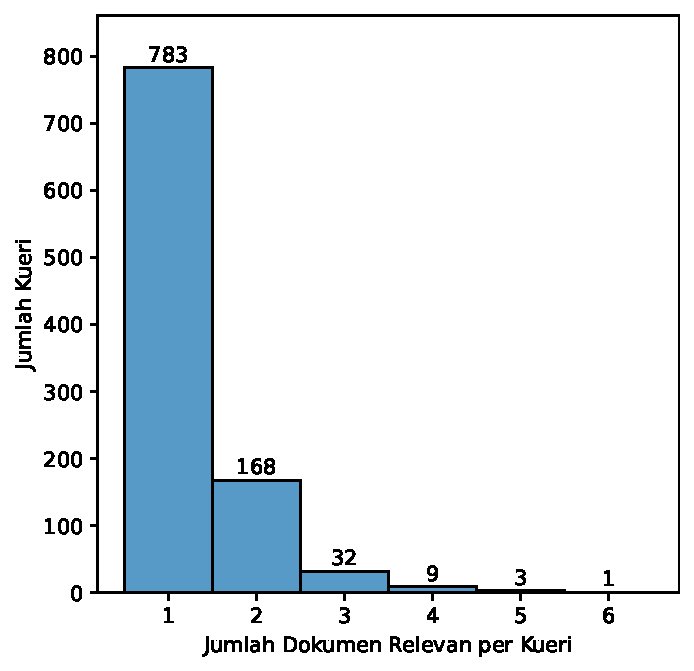
\includegraphics[scale=0.75]{assets/pdfs/Distribusi Query-Dokumen Relevan.pdf}
    \caption{Distribusi jumlah dokumen relevan untuk setiap kueri}
    \label{gambar:distribusi}
\end{figure}
Pada grafik tersebut, dapat dilihat bahwa mayoritas kueri (783) hanya memiliki 1 pasal yang relevan, diikuti oleh 168 kueri yang memiliki 2 pasal relevan dan 32 kueri dengan 3 pasal relevan. Sementara itu, kueri dengan 4 hingga 6 pasal relevan memiliki kontribusi yang kecil terhadap total jumlah kueri, masing-masing tidak lebih dari 10 jumlah kueri dan secara total hanya berkontribusi sekitar 1.31\% untuk data \training{}.
%-----------------------------------------------------------------------------%
%-----------------------------------------------------------------------------%
\section{Pengembangan Sistem \ir{}}
\label{subbab:3:Pengembangan Sistem Information Retrieval}
Peneliti melakukan pengembangan sistem \ir{} dalam bentuk \pipeline{} dengan arsitektur \cascaded{} yang terdiri dari beberapa tahap penyaringan menggunakan algoritma atau fungsi yang semakin kompleks~\citep{wang2011cascade}. \subbab{}~\ref{subbab:3:Pengembangan Sistem Information Retrieval} menjelaskan pengembangan dan pendekatan yang diambil dalam mengembangkan sistem \ir{} untuk domain legal.
%-----------------------------------------------------------------------------%
%-----------------------------------------------------------------------------%
\subsection{Definisi Tugas}
\label{subbab:3:Definisi Tugas}
Fokus dari penelitian ini adalah peningkatan efektivitas proses \retrieval{} menggunakan \hcf{} atau fitur yang dibuat secara manual seperti yang ditunjukkan pada \gambar{}~\ref{fig:posisiPenelitian}.
\begin{figure}[!ht]
    \centering
    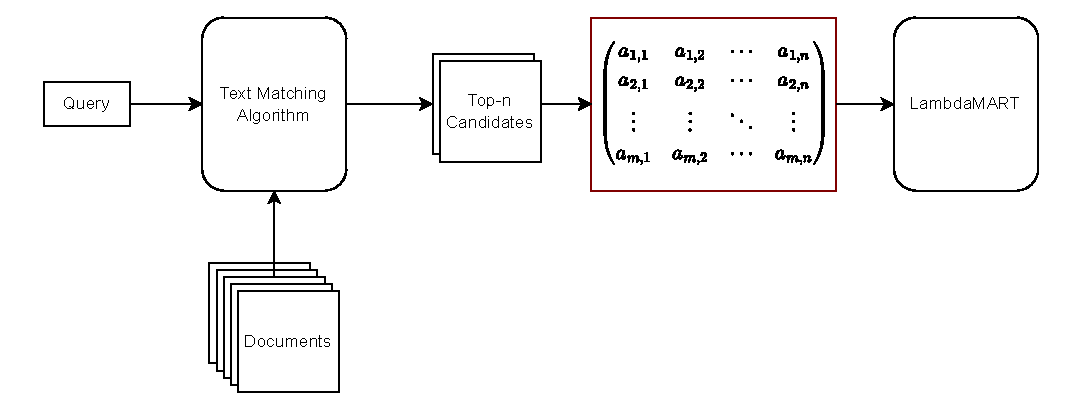
\includegraphics[scale=0.65]{assets/pdfs/PosisiPenelitian.pdf}
    \caption{Bagian dari sistem \ir{} yang akan diteliti}
    \label{fig:posisiPenelitian}
\end{figure}
Proses \retrieval{} dalam konteks ini merujuk pada pengambilan dokumen yang relevan dari sekumpulan dokumen \(D_1,D_2,...,D_k\) berdasarkan kueri \(Q\). Algoritma \txt{} \matching{} digunakan untuk mencocokkan kueri dengan dokumen-dokumen yang ada, menghasilkan urutan dokumen dari yang paling relevan hingga yang paling tidak relevan. Dengan kata lain, algoritma ini memproses kueri dan mengembalikan daftar dokumen \(D_1,D_2,...,D_k\) yang terurut berdasarkan tingkat relevansinya secara menurun. Namun, sistem \ir{} yang hanya mengandalkan pencocokan kata memiliki beberapa kekurangan, seperti tidak diperhitungkannya semantik maupun sinonim dari kata yang dicocokkan~\citep{hambarde2023information}, sehingga sebuah dokumen yang relevan memiliki kemungkinan untuk mendapatkan nilai relevansi yang rendah. Untuk mengatasi kelemahan tersebut, berbagai pendekatan telah dikembangkan demi meningkatkan efektivitas dari sistem \ir{}, seperti pengintegrasian model \ml{}~\citep{burges2010ranknet} atau model \nn{}~\citep{1223700}.

Model \nn{} tidak digunakan dalam penelitian ini karena sifatnya adalah \textit{black box} yang berarti bahwa logika dan cara kerja dari model ini tersembunyi sehingga sulit untuk memahami, melakukan verifikasi, maupun menafsirkan alasan dari keputusan yang dibuat oleh model~\citep{electronics8080832}, terutama dalam bidang \ir{}. Oleh karena itu, peneliti memilih model \ml{}, khususnya \lambdamart{}, dalam pembangunan sistem \ir{} untuk keperluan analisis fitur. Integrasi tersebut akan menerapkan arsitektur \cascaded{}~\citep{wang2011cascade} dengan seleksi 150 dokumen paling relevan oleh algoritma \txt{} \matching{} sebagai tahap pertama mengikuti penelitian terdahulu oleh \citet{nguyen2024captain}. Kemudian, dokumen-dokumen tersebut dipasangkan dengan kueri awal dan dilakukan ekstraksi fitur secara manual yang akan menjadi masukan dari \lambdamart{}. 
%-----------------------------------------------------------------------------%
%-----------------------------------------------------------------------------%
\subsection{Kajian \Base{} \Retriever{}}
\label{subbab:3:Kajian Base Retrieval}
Sebelum melakukan ekstraksi fitur dan meningkatkan efektivitas sistem dengan \lambdamart{} sebagai \reranker{}, peneliti menguji beberapa algoritma \base{} \retriever{} menggunakan data \training{}. \Base{} \retriever{} yang diuji meliputi InL2, DLH13, DFR\_BM25, BM25, DLH, TF\_IDF, LGD, PL2, IFB2, Hiemstra\_LM, DFReeKLIM, DPH, Js\_KLs, DFRee, In\_expB2, In\_expC2, LemurTF\_IDF, DFIZ, InB2, XSqrA\_M, DFIC, BB2, CoordinateMatch, DirichletLM, Tf, dan Dl. Hasil pengujian dapat ditemukan pada \tabel{}~\ref{tabel:3:base retriever}. Berdasarkan hasil tersebut, diseleksi beberapa algoritma untuk skenario penelitian yang akan dilaksanakan selanjutnya.
\begin{table}[!htb]
    \caption{Kinerja \base{} \retriever{} pada data \training{} untuk metrik \recall{}@3}
    \label{tabel:3:base retriever}
    \begin{minipage}{.5\linewidth}
      \centering
        \begin{tabular}{lr}
            \toprule
            name & R@3 \\
            \midrule
            InL2 & 0,6281 \\
            DLH13 & 0,6277 \\
            DFR\_BM25 & 0,6262 \\
            BM25 & 0,6257 \\
            DLH & 0,6247 \\
            TF\_IDF & 0,6214 \\
            LGD & 0,6207 \\
            PL2 & 0,6162 \\
            IFB2 & 0,6159 \\
            Hiemstra\_LM & 0,6154 \\
            DFReeKLIM & 0,6149 \\
            DPH & 0,6146 \\
            Js\_KLs & 0,6146 \\
            \bottomrule
        \end{tabular}
    \end{minipage}
    \begin{minipage}{.5\linewidth}
      \centering
        \begin{tabular}{lr}
            \toprule
            name & R@3 \\
            \midrule
            DFRee & 0,6139 \\
            In\_expB2 & 0,6122 \\
            In\_expC2 & 0,6087 \\
            LemurTF\_IDF & 0,6085 \\
            DFIZ & 0,6082 \\
            InB2 & 0,6060 \\
            XSqrA\_M & 0,6011 \\
            DFIC & 0,5950 \\
            BB2 & 0,5765 \\
            CoordinateMatch & 0,5501 \\
            DirichletLM & 0,5093 \\
            Tf & 0,2562 \\
            Dl & 0,1335 \\
            \bottomrule
        \end{tabular}
    \end{minipage} 
\end{table}

%-----------------------------------------------------------------------------%
%-----------------------------------------------------------------------------%
\subsection{Usulan Fitur}
\label{subbab:3:Usulan Fitur}
Dari setiap pasangan yang dikembalikan \base{} \retriever{}, akan dilakukan ekstraksi berbagai fitur untuk dianalisis penggunaannya dalam proses \reranking{}. Fitur hasil ekstraksi dapat dikategorikan ke dalam 3 kelompok, antara lain:

%-----------------------------------------------------------------------------%
\vspace{2mm}
\noindent{}\textbf{Atribut Kuantitatif Sederhana}. Atribut kuantitatif sederhana adalah fitur-fitur dasar yang dapat diekstraksi dari teks tanpa memerlukan perhitungan kompleks atau analisis mendalam. Fitur-fitur ini tidak mempertimbangkan unsur kesamaan antara kueri dan dokumen, baik secara semantik, struktural, maupun tekstual. Dalam penelitian ini, beberapa fitur kuantitatif sederhana yang dianalisis meliputi jumlah kata pada kueri \(Len(q)\), jumlah kata pada dokumen \(Len(d)\), dan selisih jumlah kata antara kueri-dokumen \(LenDiff\) yang diekspresikan secara matematis sebagai
\[LenDiff(q,d)=|Len(q)-Len(d)| \, ,\]
dengan $q$ sebagai kueri; $d$ merupakan dokumen;dan $Len(x)$ ialah jumlah kata pada $x$.

%-----------------------------------------------------------------------------%
\vspace{2mm}
\noindent{}\textbf{Skor berbasis \textit{Text Matching}}. Fitur pada kelompok ini berkaitan dengan perhitungan kesamaan antara kueri dan dokumen secara tekstual, seperti yang telah dijelaskan pada \subbab{}~\ref{subbab:2:Algoritma Text Matching}. Beberapa teknik yang akan dianalisis mencakup nilai-nilai relevansi dari \base{} \retriever{} yang dianalisis pada \subbab{}~\ref{subbab:3:Kajian Base Retrieval}. Secara umum, \base{} \retriever{} merupakan suatu algoritma pembobotan atau \weighting{}~\(w(t,d)\) untuk suatu kata atau \term{}~\(t\) pada dokumen~\(d\). Dokumen tersebut biasanya mengandung lebih dari satu \term{}, sehingga, untuk mendapatkan nilai relevansi~\(R\) suatu kueri \(q\) dengan dokumen, diperlukan penggabungan bobot dari setiap \term{}. Salah satu cara yang intuitif adalah dengan menjumlahkan bobot setiap \term{} yang dapat diekspresikan sebagai
\begin{align*}
    R(q,d)=\sum_{t\in{}q\cap{}d}w(t,d) \, .
\end{align*}
    
Nilai relevansi tersebut yang kemudian akan diekstraksi sebagai fitur untuk masukan \reranker{}. Selain nilai relevansi tersebut, dalam penelitian ini akan digunakan juga nilai kesamaan Jaccard \(J(A,B)\) dengan \(A\) dan \(B\) merupakan himpunan \term{} (kata atau frasa) yang didapatkan dari suatu teks. Dalam konteks \ir{}, nilai Jaccard tersebut dapat dikomputasi menggunakan rumus
\begin{align*}
    J(A,B)=\frac{|A\cap{}B|}{|A\cup{}B|};J(A,B)\in{}[0,1] \, ,
\end{align*}
dengan \(A\) merupakan himpunan kata \term{} dari kueri; \(B\) merupakan himpunan \term{} dari dokumen; \(|A\cap{}B|\) adalah jumlah \term{} yang berpotongan antara dokumen dengan kueri; dan \(|A\cup{}B|\) adalah jumlah gabungan \term{} unik dari dokumen dan kueri. Rumus tersebut memiliki nilai dalam interval tertutup 0 hingga 1 secara inklusif, secara spesifik bernilai 0 jika tidak ada \term{} yang sama antara kueri dengan dokumen dan bernilai 1 jika \term{} kueri dan \term{} dokumen identik. Selain menggunakan \term{} yang dibatasi pada kata untuk kesamaan Jaccard, peneliti juga menggunakan frasa dan/atau kata penting yang diekstraksi menggunakan metode yang dikembangkan oleh \citet{rose2010automatic}, yaitu RAKE. \textit{Rapid Automatic Keyword Extraction} (RAKE) adalah metode yang digunakan dalam pemrosesan bahasa alami (NLP) untuk secara otomatis mengidentifikasi kata kunci atau frasa penting pada suatu teks. Peneliti menggunakan RAKE untuk ekstraksi karena tidak diperlukan latihan khusus untuk pemakaiannya serta juga karena sifatnya yang \textit{domain-independent} dan \textit{language-independent}~\citep{rose2010automatic}. Dengan kata lain, penggunaan RAKE tidak terikat pada suatu domain tertentu maupun terbatas pada bahasa yang spesifik.

%-----------------------------------------------------------------------------%
\vspace{2mm}
\noindent{}\textbf{\textit{Semantic Similarity}}. Kelompok ini mengandung fitur-fitur yang berfokus pada kesamaan kontekstual atau semantik antara kueri dan dokumen, bukan hanya kesamaan secara tekstual. Makna atau semantik dari teks tersebut direpresentasikan dengan sebuah vektor yang diperoleh dengan memanfaatkan keluaran model \neural{} \network{}, secara khusus \tfive{} dan \bert{}. Untuk model \bert{}, peneliti menguji beberapa teknik yang diusulkan oleh \citet{devlin2018bert} dengan menggunakan kombinasi dan agregasi dari keluaran \hs{s} \bert{} tanpa \textit{fine-tuning}. Dalam penelitian ini, akan dikaji beberapa usulan \citet{devlin2018bert} dan satu usulan peneliti, yaitu  $LHS\_MEAN$, yang dinotasikan sebagai
\begin{align*}
    FHS\_CLS&=CLS(HS_{0}) \, , \\
    STLHS\_CLS&=CLS(HS_{11}) \, , \\
    LHS\_CLS&=CLS(HS_{12}) \, , \\
    SUM\_LFHS\_CLS&=CLS(HS_{9}) + CLS(HS_{10}) + CLS(HS_{11}) + CLS(HS_{12}) \, , \\
    CONCAT\_LFHS\_CLS&=CLS(HS_{9}) \oplus{} CLS(HS_{10}) \oplus{} CLS(HS_{11}) \oplus{} CLS(HS_{12}) \, , \\
    SUM\_AHS\_CLS&=\sum^{12}_{n=1} CLS(HS_{n}) \, , \\
    LHS\_MEAN&=mean(HS_{12}) \, ,
\end{align*}
dengan $HS_{n}$ merupakan vektor keluaran dari $ENC_{n}$ pada \textit{layer} ke-$n$; $CLS(HS_{n})$ adalah fungsi yang mengambil vektor \token{} pertama dari suatu \hs{} $HS_{n}$; dan \textit{mean} ialah fungsi yang menghitung rata-rata pada dimensi kedua, yaitu dimensi \token{}. Perhatikan bahwa simbol $\oplus{}$ merupakan operasi penggabungan (\textit{concatenation}) yang menambahkan suatu vektor di akhir vektor lainnya pada suatu dimensi tertentu.

Serupa halnya dengan model \bert{}, peneliti menguji beberapa teknik untuk model \tfive{} yang diusulkan oleh \citet{ni2021sentence}, yaitu dengan menggunakan rata-rata keluaran semua vektor \token{} dari \hs{} terakhir dan vektor \token{} pertama pada \hs{} terakhir yang dinotasikan dengan
\begin{align*}
    LHS\_CLS&=CLS(HS_{12}) \, ,\\
    LHS\_MEAN&=mean(HS_{12}) \, .
\end{align*}

Setelah mendapatkan representasi semantik berupa vektor dari \bert{} dan juga \tfive{}, untuk mengukur kemiripan antara kedua representasi tersebut, peneliti menggunakan \textit{cosine similarity} yang umum digunakan dalam penyelesaian tugas pemrosesan bahasa alami~\citep{wehnert2021legal,zhou2022problems}. \textit{Cosine similarity} tersebut dapat diekspresikan dengan persamaan
\begin{align*}
    cosine\_similarity(x_1,x_2)=\frac{x_1\cdot{}x_2}{max(||x_1||_2,\epsilon{})\cdot{}max(||x_2||_2,\epsilon{})} \, ,
\end{align*}
dengan \(x_n\) merupakan vektor; \(\epsilon{}\) adalah konstanta yang sangat kecil (\(\expnumber{1}{-8}\)); dan \(||x_n||_2\) sebagai norma \textit{Euclidean} dari vektor \(x_n\). Konstanta \(\epsilon{}\) tersebut ditambahkan untuk mencegah terjadinya masalah komputasi, yaitu pembagian dengan 0.

%-----------------------------------------------------------------------------%
\subsection{Evaluasi Model}
\label{subbab:3:Evaluasi Model}
Evaluasi yang dilakukan terhadap model dalam penelitian ini mencakup evaluasi hasil menggunakan metrik dan evaluasi korelasi menggunakan koefisien korelasi \textit{pearson}. Metrik, dalam hal ini, akan digunakan untuk membandingkan kinerja antar sistem. Sementara itu, koefisien \textit{pearson} akan dimanfaatkan untuk menentukan hubungan linear dari dua buah variabel yang akan berguna untuk menyelidiki korelasi antara \cutoff{} dengan efektivitas sistem \ir{}.

\vspace{2mm}
\noindent{}\textbf{Metrik Evaluasi}.
\label{bagian:Metrik Evaluasi}
Model dievaluasi menggunakan metrik yang dihitung berdasarkan urutan dokumen yang dikembalikan. Dari grafik pada \gambar{}~\ref{gambar:distribusi}, didapatkan distribusi yang memiliki rata-rata 1.2771 dan median 1 serta 98.69\% dari kueri tersebut hanya memiliki paling banyak 3 dokumen yang relevan. Karena tujuan dari perancangan sistem \ir{} dalam penelitian ini adalah memperbanyak dokumen relevan yang ditemui pada dokumen teratas untuk keperluan evaluasi oleh badan hukum, maka peneliti menentukan metrik \recall{}, secara spesifik pada \cutoff{} 3 atau pada 3 dokumen teratas untuk mengevaluasi kinerja sistem tersebut. Metrik \recall{} dapat dihitung menggunakan rumus
\begin{align*}
    R@k=\frac{TP}{TP+FN} \, ,
\end{align*}
dengan \(R@k\) adalah \recall{} pada \(k\) dokumen teratas; TP merupakan jumlah dokumen diantara $k$ dokumen teratas yang diketahui relevan; dan FN ialah jumlah dokumen relevan yang gagal dikembalikan diantara \(k\) dokumen teratas tersebut. Selain itu, terdapat beberapa metrik yang digunakan untuk keperluan analisis lebih lanjut. Pertama, \textit{precision} yang dapat dihitung sebagai
\[
P@k=\frac{TP}{TP+FP} \, ,
\]
dengan $P@k$ merupakan \textit{precision} pada $k$ dokumen teratas; dan FP ialah jumlah dokumen tidak relevan yang dikembalikan pada $k$ dokumen teratas. Kedua, \textit{reciprocal rank} ($recip\_rank$) yang dinotasikan sebagai
\[
recip\_rank=\frac{1}{rank} \, ,
\]
dengan $rank$ merupakan peringkat dari dokumen relevan teratas. Kemudian, \textit{Mean Average Precision} (MAP) yang dirumuskan sebagai
\begin{align*}
    MAP&=\frac{1}{Q} \sum_{q=1}^Q AP(q) \, ,\\
    AP(q)&=\frac{1}{R} \sum_{n=1}^N P@n \cdot rel@n \, ,
\end{align*}
dengan $Q$ merupakan jumlah kueri yang dievaluasi; $AP(q)$ ialah \textit{average precision} untuk suatu kueri $q$; $R$ adalah jumlah dokumen relevan yang diketahui; $rel@n$ merupakan relevansi dokumen pada posisi $n$; $N$ sebagai jumlah dokumen yang dikembalikan;  Terakhir, terdapat metrik NDCG yang telah didefinisikan pada~\subbab{}~\ref{subbab:2:LambdaRank}

\vspace{2mm}
\noindent{}\textbf{Korelasi \textit{Pearson}}.
\label{bagian:Korelasi Pearson}
Korelasi \textit{pearson} $r$ adalah suatu perhitungan statistik yang mengevaluasi kekuatan dan hubungan linear sepasang variabel. Nilai \textit{pearson} tersebut dapat diperoleh dengan perhitungan
\[
r=\frac{n\sum{}xy-(\sum{}x)(\sum{}y)}{\sqrt{(n\sum{}x^2-(\sum{}x)^2)(n\sum{}y^2-(\sum{}y)^2)}} \, ,
\]
dengan $n$ merupakan jumlah data yang diamati; serta $x$ dan $y$ adalah variabel data yang ingin diselidiki korelasinya.

%-----------------------------------------------------------------------------%
\subsection{Feature Importance}
\label{subbab:3:Feature Importance}
% akan dimanfaatkan sebagai tolok ukur penentuan karakteristik atau fitur yang dapat membantu klasifikasi relevansi antara sepasang kueri dan dokumen.
Evaluasi pemanfaatan fitur merupakan aspek penting dalam mengukur kinerja model, selain dari hasil yang diperoleh melalui metrik. Nilai \feature{} \importance{} akan digunakan sebagai tolok ukur penentuan karakteristik atau fitur yang dapat bermanfaat dalam menentukan nilai relevansi antara sepasang kueri dan dokumen. Dalam penelitian ini, nilai \feature{} \importance{} dari \lambdamart{} akan digunakan untuk evaluasi pemanfaatan fitur. Model \reranker{} tersebut dipilih karena kemampuannya yang unik dalam mengorbankan kinerja pada kueri tertentu untuk meningkatkan kinerja keseluruhan melalui proses seleksi \textit{split} dan penentuan nilai \textit{leaf}~\citep{burges2010ranknet}. Proses seleksi ini memungkinkan model untuk memilih fitur-fitur yang paling relevan dalam setiap tahap pemisahan data, yang kemudian digunakan untuk mengidentifikasi fitur mana yang paling sering digunakan. Dengan menganalisis frekuensi penggunaan fitur ini, peneliti dapat mengungkap karakteristik penting yang berkontribusi signifikan terhadap tugas penentuan relevansi dokumen legal. Analisis ini memberikan wawasan mendalam mengenai fitur-fitur kunci yang mempengaruhi keputusan model, serta membantu dalam pemahaman yang lebih baik tentang cara kerja model dan langkah-langkah yang dapat diambil untuk meningkatkan kinerjanya lebih lanjut.
% Selain evaluasi hasil menggunakan metrik, peneliti juga melakukan evaluasi pemanfaatan fitur oleh model. Model \reranker{} yang akan digunakan untuk analisis adalah \lambdamart{}, terutama karena kemampuannya dalam memilih untuk mengorbankan kinerja pada kueri tertentu namun meningkatkan kinerja secara keseluruhan dengan melakukan seleksi \textit{split} dan nilai \textit{leaf}~\citep{burges2010ranknet}. Peneliti memanfaatkan hasil seleksi tersebut untuk melakukan analisis frekuensi penggunaan fitur yang menggambarkan karakteristik penting dalam tugas klasifikasi relevansi dokumen legal.
%-----------------------------------------------------------------------------%




% %-----------------------------------------------------------------------------%
% % baseline yang baik untuk \ir{} pada domain legal, yaitu BM25~\citep{DBLP:journals/corr/abs-2105-05686} dan TF-IDF~.
% %-----------------------------------------------------------------------------%



% %-----------------------------------------------------------------------------%
% \section{Analisis Fitur}
% \label{subbab:3:analisisFitur}




% \subsection{Seleksi K-Dokumen Paling Relevan}
% \label{subbab:3:seleksiNDokumenPalingRelevan}

% Proses seleksi k-dokumen paling relevan dilakukan dengan menghitung nilai relevansi setiap pasangan \query{}-dokumen menurut algoritma \base{} \retrieval{}. Setelah mendapat nilai dari setiap pasang, dokumen tersebut akan diurutkan berdasarkan nilai relevansi secara menurun dan diseleksi sejumlah maksimal k-dokumen yang paling relevan. Dokumen yang berhasil dikembalikan oleh proses tersebut kemudian diekstraksi fitur-fiturnya sebagai masukan untuk \reranker{}. Dalam penelitian ini, akan digunakan nilai \cutoff{} \(k=150\) mengikuti \citet{nguyen2024captain} yang berhasil mendapatkan kinerja \(f2\) terbaik pada \COLIEE{} 2023, dengan nilai \(f2\) didapat dari persamaan
% \begin{align*}
% f2=\frac{5 × precision × recall}{4 × precision + recall}
% \end{align*}

% \subsection{Ekstraksi Fitur}
% \label{subbab:3:ekstraksiFitur}

% Dari setiap pasangan yang dikembalikan \base{} \retriever{}, akan dilakukan ekstraksi berbagai fitur untuk dianalisis penggunaannya dalam proses \reranking{}. Fitur hasil ekstraksi dapat dikategorisasikan ke dalam 3 kelompok, antara lain:

% \begin{itemize}[label={}]
%     \item~\textbf{Atribut Kuantitatif Sederhana}. Atribut kuantitatif sederhana adalah fitur-fitur dasar yang dapat diekstraksi dari teks tanpa memerlukan perhitungan yang kompleks atau analisis mendalam. Fitur dalam kelompok ini tidak mempertimbangkan unsur kesamaan antara query dan dokumen, baik secara semantik, struktural, maupun tekstual. Fitur yang akan dianalisis dalam penelitian ini meliputi jumlah kata pada \query{}, jumlah kata pada dokumen, dan Selisih jumlah kata antara \query{}-dokumen.
    
%     \item~\textbf{\Txt{} \Matching{}}. Fitur pada kelompok ini berkaitan dengan perhitungan kesamaan antara \query{} dan dokumen secara tekstual. Beberapa teknik yang akan dianalisis mencakup nilai relevansi dari \base{} \retriever{} yang dianalisis pada \bab~\ref{subbab:3:analisisBaseRetrieval}, nilai Jaccard dari \query{} dan dokumen, serta nilai Jaccard dari hasil ekstraksi RAKE \query{} dan dokumen.
    
%     \item~\textbf{\Semantic{} \Similarity{}}. Fitur yang termasuk dalam kelompok ini berfokus pada kesamaan kontekstual atau semantik antara \query{} dan dokumen, bukan hanya kesamaan secara tekstual. Makna atau semantik dari teks tersebut direpresentasikan dengan sebuah vektor yang diperoleh dengan memanfaatkan beberapa model \neural{} \network{}, yaitu \tfive{} dan \bert{}. Untuk representasi vektor yang digunakan sebagai fitur dari kedua model tersebut, peneliti menguji teknik ekstraksi \citet{devlin2018bert} untuk \bert{} serta beberapa teknik ekstraksi \citet{ni2021sentence} untuk \tfive{}.
% \end{itemize}

% \todo{Ini juga kah pak?
%     \begin{itemize}
%         \item Visualisasi vektor mana yang diambil dari BERT~\citep{devlin2018bert}
%         \item Jelasin visualisasi (\citet{devlin2018bert} ngapain)
%         \item Visualisasi vektor mana yang diambil dari T5~\citep{ni2021sentence}
%         \item Jelasin visualisasi (\citet{ni2021sentence} ngapain)
%     \end{itemize}}



% \subsection{\Reranking{} dengan \lambdamart{}}
% \label{subbab:3:rerankingDenganLambdamart}

% Setelah didapat hasil ekstraksi fitur, sebuah \reranker{} akan digunakan untuk proses \reranking{} dokumen agar dokumen-dokumen yang relevan namun memiliki peringkat yang rendah akan mendapat peringkat yang lebih baik. Dalam penelitian ini, \reranker{} yang akan digunakan adalah \lambdamart{} karena kemampuannya dalam memilih untuk mengorbankan kinerja pada \query{} tertentu namun meningkatkan kinerja secara keseluruhan dengan melakukan seleksi \textit{split} dan nilai \textit{leaf} \citep{burges2010ranknet}.



% \subsection{\Training{} dan Eksperimen}
% \label{subbab:3:rerankerTrainingDanEksperimen}

% Seperti yang telah dijelaskan pada \bab~\ref{subbab:3:analisisFitur}, bahwa akan dirancang sebuah \pipeline{} untuk masing-masing \base{} \retriever{} yang telah ditentukan pada \bab~\ref{subbab:3:analisisBaseRetrieval}, maka akan diperoleh sebanyak 5 \base{} \retriever{} dan 5 sistem \ir{} dengan \reranker{} \lambdamart{}. Model \lambdamart{} akan dilatih menggunakan seluruh fitur pada \bab~\ref{subbab:3:ekstraksiFitur} dan akan dievaluasi kinerjanya dengan membandingkan \base{} \retriever{} yang sesuai. Pelatihan model \lambdamart{} dan evaluasi akan dilakukan dengan teknik \textit{5-fold cross validation} agar diperoleh hasil evaluasi yang dapat mewakilkan kinerja sistem yang sesungguhnya.
% %-----------------------------------------------------------------------------%



% %-----------------------------------------------------------------------------%
% \section{Analisis \Cutoff{} \base{} \retrieval{}}
% \label{subbab:3:analisisCutoffBaseRetrieval}

% Pengujian juga dilakukan pada beberapa \cutoff{} untuk menentukan batasan sedemikian sehingga sistem \ir{} domain legal yang akan dirancang dapat berfungsi dengan efektif dan efisien. Proses pengujian dilakukan seperti yang telah dijelaskan pada \bab~\ref{subbab:3:analisisFitur} dengan perbedaan hanya pada jumlah dokumen yang dikembalikan (\cutoff{}) oleh \base{} \retriever{}. Pada pengujian ini, peneliti memiliki hipotesis bahwa \cutoff{} memiliki korelasi positif dengan kinerja model dengan pengaruh yang semakin kecil dengan bertambahnya \cutoff{} sehingga membentuk suatu kurva asimtot.
% %-----------------------------------------------------------------------------%



% %-----------------------------------------------------------------------------%
% \section{\Incremental{} \Ablation{} \Learning{}}
% \label{subbab:3:ablationLearning}

% Setelah mendapatkan sistem \ir{} dengan \cutoff{} yang paling efektif dari \bab~\ref{subbab:3:analisisCutoffBaseRetrieval}, peneliti akan melakukan analisis pengaruh jumlah fitur terhadap kinerja sistem. Pengujian dilakukan dengan menambahkan jumlah fitur yang digunakan sistem secara inkremental dan melakukan analisis perubahan kinerja sistem. Proses penambahan fitur dilakukan secara terurut dimulai dari fitur dengan \feature{} \importance{} paling tinggi sampai ke yang paling rendah. Dengan melakukan \incremental{} \ablation{} \learning{}, peneliti dapat menentukan jumlah fitur yang efisien untuk perancangan sistem \ir{} domain legal.
% %-----------------------------------------------------------------------------%